\chapter{Il teorema di Bayes}
\label{chapter:bayes_theo} 


Il teorema di Bayes ha un ruolo centrale nella statistica Bayesiana, anche se viene utilizzato anche dall'approccio frequentista.
Prima di esaminare il teorema di Bayes introdurremo una sua componente, ovvero il teorema della probabilità totale.

\section{Il teorema della probabilità totale}
\label{sec:tot_prob_theorem}

Il teorema della probabilità totale fa uso della legge della probabilità composta \eqref{eq:probcomposte} per calcolare le probabilità di casi più complessi di quelli considerati fino ad ora. 
La notazione sembra complessa, ma l'idea sottostante è semplice. 
Discutiamo qui il teorema della probabilità totale considerando il caso di una partizione dello spazio campionario in tre sottoinsiemi. 
È facile estendere tale situazione al caso di una partizione in un qualunque numero di sottoinsiemi.
\begin{teorema}
Sia $\{A_1, A_2, A_3\}$ una partizione dello spazio campionario $\Omega$. Se $E$ è un qualunque altro evento, allora:
\begin{equation}
P(E) = P(E \cap A_1) + P(E \cap A_2) + P(E \cap A_3) \notag
\label{eq:prob_total_1a}
\end{equation}
\noindent ovvero
\begin{equation}
P(E) = P(E \mid A_1) P(A_1) + P (E \mid A_2) P(A_2) + P(E \mid A_3) P(A_3).
\label{eq:prob_total_1b}
\end{equation}
\end{teorema}

Il teorema della probabilità totale afferma che, se l'evento $E$ è costituito da tutti gli eventi elementari in $E \cap A_1$, $E \cap A_2$ e $E \cap A_3$, allora la probabilità $P(E)$ è data dalla somma delle probabilità di queti tre eventi. 
Ciò è illustrato nella figura seguente.

\begin{figure}[h!]
\centering
\begin{tikzpicture}
\tikzset{
    myrectangle/.style={
        draw=black,
        minimum width=4cm,
        minimum height=2cm,
    },
    A/.style={
        draw=gray,
    },
    E/.style={
        draw=gray,
    },
    >=stealth,
    node distance=1cm and 1cm,
}

    \node[myrectangle] (left) {};
    \node[myrectangle] (right) [right=of left] {};
    \path (left.south east) -- coordinate (tmp) (right.south west);
    \node[myrectangle] (bottom) [below=of tmp] {};

    % "contents" of left node
    \path (left.west) -- node[pos=.25] {$A_1$} (left.east);
    \path (left.west) -- node[pos=.5] {$A_2$} (left.east);
    \path (left.west) -- node[pos=.75] {$A_3$} (left.east);

    \draw[A] ($(left.north west) ! .4 ! (left.north east)$) -- ($(left.south west) ! .35 ! (left.south east)$);
    \draw[A] ($(left.north west) ! .6 ! (left.north east)$) -- ($(left.south west) ! .66 ! (left.south east)$);

    % "contents" of right node
    \draw[E] (right.center) ellipse [x radius=1.5cm, y radius=0.75cm] node {$E$};

    % "contents" of bottom node
    \path (bottom.west) -- node[pos=.25] {\scriptsize $E\cap A_1$} (bottom.east);
    \path (bottom.west) -- node[pos=.5] {\scriptsize $E \cap A_2$} (bottom.east);
    \path (bottom.west) -- node[pos=.75] {\scriptsize $E \cap A_3$} (bottom.east);

    \draw[A] ($(bottom.north west) ! .4 ! (bottom.north east)$) -- ($(bottom.south west) ! .35 ! (bottom.south east)$);
    \draw[A] ($(bottom.north west) ! .6 ! (bottom.north east)$) -- ($(bottom.south west) ! .66 ! (bottom.south east)$);

    \draw[E] (bottom.center) ellipse [x radius=1.5cm, y radius=0.75cm];

    % arrows
    \begin{scope}[
        shorten >=.2cm,
        shorten <=.2cm,
    ]
        \draw[->, black] (left) -- (bottom);
        \draw[->, black] (right) -- (bottom);
    \end{scope}

    % labels on top
    \node at (left.north east) [anchor=south east] {$\Omega$};
    \node at (right.north east) [anchor=south east] {$\Omega$};
    \node at (bottom.north east) [anchor=south east] {$\Omega$};
\end{tikzpicture}
\end{figure}
\bigskip


\begin{exmp}
\label{exmp:3urne}
Si considerino tre urne, ciascuna delle quali contiene 100 palline:
\begin{itemize}
\item Urna 1: 75 palline rosse e 25 palline blu,
\item Urna 2: 60 palline rosse e 40 palline blu,
\item Urna 3: 45 palline rosse e 55 palline blu.
\end{itemize}
Una pallina viene estratta a caso da un'urna anch'essa scelta a caso.
Qual è la probabilità che la pallina estratta sia di colore rosso?
\end{exmp}

\begin{solu}
Sia $R$ l'evento \enquote{la pallina estratta è rossa} e sia $U_i$ l'evento che corrisponde alla scelta dell'$i$-esima urna.
Sappiamo che
\[
P(R \mid U_1) = 0.75, \qquad P(R \mid U_2) = 0.60, \qquad P(R \mid U_3) = 0.45.
\]
Gli eventi $U_1$, $U_2$ e $U_3$ costituiscono una partizione dello spazio campionario in quanto $U_1$, $U_2$ e $U_3$ sono eventi mutualmente esclusivi ed esaustivi, $P(U_1 \cup U_2 \cup U_3) = 1.0$.    
In base al teorema della probabilità totale, la probabilità di estrarre una pallina rossa è
\begin{align}
P(R) &= P(R \mid U_1)P(U_1)+P(R \mid U_2)P(U_2)+P(R \mid U_3)P(U_3)\notag\\
&= 0.75 \cdot \frac{1}{3}+0.60 \cdot \frac{1}{3}+0.45 \cdot \frac{1}{3} =0.60.\notag
\end{align}

\end{solu}


\begin{exmp}
\label{exmp:urna_5r2v}
Consideriamo un'urna che contiene 5 palline rosse e 2 palline verdi. Due palline vengono estratte, una dopo l'altra. Vogliamo sapere la probabilità dell'evento ``la seconda pallina estratta è rossa''. 
\end{exmp}

\begin{solu}
Lo spazio campionario è $\Omega = \{RR, RV, VR, VV\}$. Chiamiamo $R_1$ l'evento \enquote{la prima pallina estratta è rossa}, $V_1$ l'evento \enquote{la prima pallina estratta è verde}, $R_2$ l'evento \enquote{la seconda pallina estratta è rossa} e $V_2$ l'evento \enquote{la seconda pallina estratta è verde}. 
Dobbiamo trovare $P(R_2)$ e possiamo risolvere il problema usando il teorema della probabilità totale~\eqref{eq:prob_total_1b}:

\begin{align}
P(R_2) &= P(R_2 \mid R_1) P(R_1) + P(R_2 \mid V_1)P(V_1)\notag\\
&= \frac{4}{6} \cdot \frac{5}{7} + \frac{5}{6} \cdot \frac{2}{7} = \frac{30}{42} = \frac{5}{7}.\notag
\end{align}
Se la prima estrazione è quella di una pallina rossa, nell'urna restano 4 palline rosse e due verdi, dunque, la probabilità che la seconda estrazione produca una  pallina rossa è uguale a 4/6.
La probabilità di una pallina rossa nella prima estrazione è 5/7.
Se la prima estrazione è quella di una pallina verde, nell'urna restano 5 palline rosse e una pallina verde, dunque, la probabilità che la seconda estrazione produca una pallina rossa è uguale a 5/6.
La probabilità di una pallina verde nella prima estrazione è 2/7.
\end{solu}


%%--------------------------------------------------------------------
%\subsection{Il diagramma ad albero}
%\label{sec:tree_diagram}
%
%I diagrammi ad albero consentono di semplificare la descrizione dei possibili risultati ottenuti a partire da un esperimento a più stadi:
%\begin{itemize}
%\item per ogni stadio ci sono tanti rami quante sono le possibilità,
%\item il numero totale dei percorsi rappresenta il numero totale degli eventi possibili,
%\item ad ogni percorso è associata la probabilità corrispondente all'evento rappresentato.
%\end{itemize}
%
%\begin{exmp}
%Possiamo rappresentare il diagramma ad albero per l'esempio~\ref{exmp:urna_5r2v} come indicato di seguito. 
%
%\bigskip
%
%% Set the overall layout of the tree
%\tikzstyle{level 1}=[level distance=3.5cm, sibling distance=3.5cm]
%\tikzstyle{level 2}=[level distance=3.5cm, sibling distance=2cm]
%
%% Define styles for bags and leafs
%\tikzstyle{bag} = [text width=4em, text centered]
%\tikzstyle{end} = [circle, minimum width=3pt,fill, inner sep=0pt]
%
%% The sloped option gives rotated edge labels. Personally
%% I find sloped labels a bit difficult to read. Remove the sloped options
%% to get horizontal labels. 
%\begin{tikzpicture}[grow=right, sloped]
%\node[bag] {Urna 1 $5R, 2V$}
%    child {
%        node[bag] {Urna 2 $5R, 1V$}        
%            child {
%                node[end, label=right:
%                    {$P(V_1\cap V_2)=\frac{2}{7}\cdot\frac{1}{6}$}] {}
%                edge from parent
%                node[above] {$V$}
%                node[below]  {$\frac{1}{6}$}
%            }
%            child {
%                node[end, label=right:
%                    {$P(V_1\cap R_2)=\frac{2}{7}\cdot\frac{5}{6}$}] {}
%                edge from parent
%                node[above] {$R$}
%                node[below]  {$\frac{5}{6}$} %
%            }
%            edge from parent 
%            node[above] {$V$}
%            node[below]  {$\frac{2}{7}$}
%    }
%    child {
%        node[bag] {Urna 2 $4R, 2V$}        
%        child {
%                node[end, label=right:
%                    {$P(R_1\cap V_2)=\frac{5}{7}\cdot\frac{2}{6}$}] {}
%                edge from parent
%                node[above] {$V$}
%                node[below]  {$\frac{2}{6}$}
%            }
%            child {
%                node[end, label=right:
%                    {$P(R_1\cap R_2)=\frac{5}{7}\cdot\frac{4}{6}$}] {}
%                edge from parent
%                node[above] {$R$}
%                node[below]  {$\frac{4}{6}$}
%            }
%        edge from parent         
%            node[above] {$R$}
%            node[below]  {$\frac{5}{7}$}
%    };
%\end{tikzpicture}
%
%\bigskip
%La probabilità di giungere a ciascuno dei nodi del diagramma è data dal prodotto delle probabilità che si incontrano lungo il percorso che porta a quel nodo, dato che gli eventi sono indipendenti. 
%Per esempio, la probabilità dell'evento ``pallina verde nella prima estrazione e pallina rossa nella seconda estrazione'' è $\frac{2}{7} \cdot \frac{5}{6}$.
%La probabilità di ottenere una pallina rossa nella seconda estrazione è invece uguale alla probabilità dell'evento $\{R_1 \cap R_2\} \cup \{V_1 \cap R_2\}$, ovvero 
%\[
%P(R_2) = \frac{5}{7} \cdot\frac{4}{6} + \frac{2}{7} \cdot\frac{5}{6} = \frac{5}{7}. 
%\]
%\end{exmp}
%

%--------------------------------------------------------------------
\section{Il teorema della probabilità delle cause}
\label{sec:bayes_theorem}

Il teorema di Bayes rappresenta uno dei fondamenti della teoria della probabilità e della statistica. 
Lo presentiamo qui considerando prima un caso specifico per poi descriverlo nella sua forma più generale.

Sia $\{A_1, A_2\}$ una partizione dello spazio campionario $\Omega$. 
Consideriamo un terzo evento $E \subset \Omega$ con probabilità non nulla di cui si conoscono le probabilità condizionate rispetto ad $A_1$ e a $A_2$, ovvero $P(E \mid A_1)$ e $P(E \mid A_2)$. 
È chiaro per le ipotesi fatte che se si verifica $E$ deve anche essersi verificato almeno uno degli eventi $A_1$ e $A_2$. 
Supponendo che si sia verificato l'evento $E$, ci chiediamo: qual è la probabilità che si sia verificato $A_1$ piuttosto che $A_2$? 
\begin{figure}[h!]
\centering
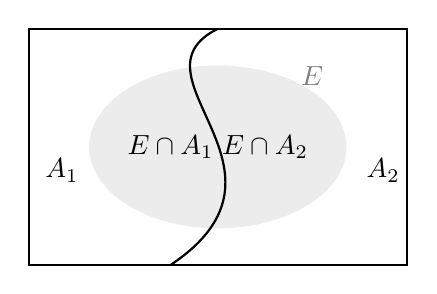
\begin{tikzpicture}[scale=.6]
  % \draw[thick] (0,0) -- (0,5) -- (8,5) -- (8,0) -- (0,0);
  \draw[thick] (0,0) rectangle (8,5);
  \draw[thick, color=gray!15, fill] (4,2.5) ellipse (2.7cm and 1.7cm);
  \draw[thick] (3,0) .. controls (6,2) and (2,4) .. (4,5);
  \node (n1) at (6,4) {\textcolor{gray}{$E$}};
  \node (n2) at (0.7,2) {$A_1$};
  \node (n2) at (3,2.5) {$E\cap A_1$};
  \node (n2) at (5,2.5) {$E\cap A_2$};
  \node (n3) at (7.5,2) {$A_2$};
\end{tikzpicture}
\end{figure}

\noindent
Per rispondere alla domanda precedente scriviamo:
\begin{align}
P(A_1 \mid E) &= \frac{P(E \cap A_1)}{P(E)}\notag\\ 
&= \frac{P(E \mid A_1)P(A_1)}{P(E)}\notag.
\end{align}
Sapendo che $E = (E \cap A_1) \cup (E \cap A_2)$ e che  $A_1$ e $A_2$ sono eventi disgiunti, ovvero $A_1 \cap A_2 = \emptyset$, ne segue che possiamo calcolare $P(E)$ utilizzando il teorema della probabilità totale:
\begin{align}
P(E) &= P(E \cap A_1) + P(E \cap A_2)\notag\\ 
&= P(E \mid A_1)P(A_1) + P(E \mid A_2)P(A_2).\notag
\end{align}
Sostituendo il risultato precedente nella formula della probabilità condizionata $P(A_1 \mid E)$ otteniamo:
\begin{equation}
P(A_1 \mid E) = \frac{P(E \mid A_1)P(A_1)}{P(E \mid A_1)P(A_1) + P(E \mid A_2)P(A_2)}.
\label{eq:bayes1}
\end{equation}
La~\eqref{eq:bayes1} si generalizza facilmente al caso di più di due eventi disgiunti, come indicato di seguito.

\begin{teorema}
Siano $A_1$, $A_2,$ \dots, $A_n$ $n$ eventi disgiunti con $P(A_i) > 0$ e tali che $\bigcup_{i=1}^{n} A_i = \Omega$.  
Per l'evento $E \subset \Omega$  con $P(E) > 0$, abbiamo
\begin{equation}
P(A_j \mid E) = \frac{P(E \mid A_j)P(A_j)}{\sum_{i=1}^{n}P(E \mid A_i)P(A_i)}.
\label{eq:bayes2}
\end{equation}
\end{teorema}
\noindent
La formula~\eqref{eq:bayes2} prende il nome di \emph{Teorema di Bayes} e mostra che la conoscenza del verificarsi dell'evento $E$ modifica la probabilità che abbiamo attribuito all'evento $A_j$.


%\subsection{Test diagnostici}
%
%Una applicazione del teorema di Bayes in campo bio-medico è quella ai test diagnostici. 
%Il risultato di un test si dice positivo quando indica la presenza della malattia, negativo quando la esclude. 
%Tuttavia, il test può fornire risultati errati e, di conseguenza, si possono presentare quattro situazioni distinte:
%\begin{enumerate}
%\item la malattia è presente e il test è positivo (\emph{vero-positivo});
%\item la malattia è presente ma il test è negativo (\emph{falso-negativo});
%\item la malattia è assente ma il test è positivo (\emph{falso-positivo});
%\item la malattia è assente e il test è negativo (\emph{vero-negativo}).
%\end{enumerate}
%Il test diagnostico fornisce un risultato corretto nei casi 1 e 4  mentre  commette un errore nei casi 2 e 3. 
%
%Supponiamo di sottoporre  un individuo ad un test diagnostico e indichiamo  con $M$  l'evento \enquote{la malattia è presente} e con $M^\complement$ l'evento \enquote{la malattia è assente}; indichiamo inoltre con $+$ l'evento \enquote{il test è positivo} e con $-$ l'evento \enquote{il test è negativo}. 
%Il tasso dei risultati falsi-positivi è dato da $P(+ \mid M^\complement)$ mentre il tasso dei risultati falsi-negativi è dato da $P(- \mid M)$.
%\begin{defn}
%Si dice \emph{sensibilità} del test la probabilità di un vero-positivo: 
%\begin{equation}
%P(+ \mid M) =  1 - P(- \mid M).\notag
%\end{equation}
%\end{defn}
%\begin{defn}
%Si dice \emph{specificità} del test la probabilità di un vero-negativo: 
%\begin{equation}
%P(- \mid M^\complement) =  1 - P(+ \mid M^\complement).\notag
%\end{equation}
%\end{defn}
%La sensibilità e la specificità sono caratteristiche intrinseche del test che ne descrivono la capacità diagnostica. 
%I dati sulla sensibilità e specificità vengono solitamente forniti dai produttori dei test. 
%Nella pratica quotidiana, invece, la domanda di interesse non è tanto: ``se un individuo è malato quanto è probabile che il test risulti positivo'' o viceversa ``se un individuo è sano quanto è probabile che il test risulti negativo'' ma piuttosto: ``se un test risulta positivo, quanto è probabile che l'individuo abbia davvero la malattia?'' oppure ``se un test risulta negativo, quanto è probabile che l'individuo sia veramente sano?'' 
%Per rispondere a tali domande procediamo come segue.
%
%Supponiamo di conoscere la prevalenza della malattia nella popolazione, ovvero $P(M)$. 
%Ne segue che $P (M^\complement) = 1 - P(M)$ è la probabilità che un individuo scelto a caso sia sano. 
%Il problema che ci poniamo è: ``qual è la probabilità che un individuo risultato positivo al test sia effettivamente malato?'' 
%Per il Teorema di Bayes si ha che
%\begin{align}
%P(M \mid +) &= \frac{P(+ \mid M) P(M)}{P(+ \mid M) P(M) + P(+ \mid M^\complement) P(M^\complement)}\notag\\ 
%&= \frac{\text{sensibilità} \cdot \text{prevalenza}}{\text{sensibilità} \cdot \text{prevalenza} + (1-\text{specificità}) \cdot (1 - \text{prevalenza})}.
%\label{eq:bayes_test_diagnostici}
%\end{align}
%
%\begin{figure}[h!]
%\centering
%\begin{tikzpicture}[scale=.6]
%  % \draw[thick] (0,0) -- (0,5) -- (8,5) -- (8,0) -- (0,0);
%  \draw[thick] (0,0) rectangle (8,5);
%  \draw[thick, color=gray!15, fill] (4,2.5) ellipse (2.7cm and 1.7cm);
%  \draw[thick] (3,0) .. controls (6,2) and (2,4) .. (4,5);
%  \node (n1) at (6,4) {\textcolor{gray}{$+$}};
%  \node (n2) at (0.7,2) {$M$};
%  \node (n2) at (2.6,2.5) {$+\cap M$};
%  \node (n2) at (5.4,2.5) {$+\cap M^\complement$};
%  \node (n3) at (7.5,2) {$M^\complement$};
%\end{tikzpicture}
%\end{figure}
%
%Il teorema di Bayes consente, conoscendo la prevalenza di una malattia, e la sensibilità e la specificità di un test per la sua diagnosi, di calcolare la probabilità di malattia in caso di test positivo (o la probabilità di assenza della malattia in caso di test negativo). 
%Fornisce dunque le basi della razionalità nella decisione che viene presa sulla base dei dati a disposizione. 
%L'equazione~\eqref{eq:bayes_test_diagnostici} rende chiaro che, per conoscere il \emph{valore predittivo del test} $P(M \mid \mathcal{H}^+)$, non basta che siano note la specificità e la sensibilità del test, ma è anche necessario conoscere la prevalenza della malattia nella popolazione, ovvero $P(M)$. 
%Il punto importante è che una bassa prevalenza della malattia nella popolazione, unita all'errore di misurazione del test, ha l'effetto di aumentare l'incertezza dell'interpretazione dei risultati del  test diagnostico.
%
%In maniera parallela a ciò che abbiamo scritto in precedenza possiamo anche calcolare la probabilità che la malattia sia assente se il test dà un risultato negativo:
%\begin{align}
%P(M^\complement \mid -) &= \frac{P(- \mid M^\complement) P(M^\complement)}{P(- \mid M^\complement) P(M^\complement) + P(- \mid M) P(M)}\notag\\ 
%&= \frac{\text{specificità} \cdot (1 - \text{prevalenza})}{\text{specificità} \cdot (1 - \text{prevalenza}) + (1-\text{sensibilità}) \cdot \text{prevalenza}}.
%\label{eq:non_malat_test_neg}
%\end{align}
%La probabilità che la malattia sia assente in un soggetto con un test negativo, $P(M^\complement \mid -)$, è definita come il \emph{valore predittivo del test negativo}. 
%
%
%
%\begin{exmp}
%I test HIV di quarta generazione hanno una sensitività del $99.9$\% e una specificità del $99.5$\%. 
%Nel 2015 il numero di individui infetti da HIV in Italia è stato stimato essere pari a $\num{140000}$, con una  prevalenza della malattia pari a $\num{140000 / 60000000} \approx 0.0023$, ovvero a circa il $2.3$ per mille della popolazione totale. 
%Si trovi la probabilità che un individuo risultato positivo al test sia infetto da HIV.
%\end{exmp}
%
%\begin{solu}
%La probabilità che un individuo sia infetto da HIV, essendo risultato positivo al test, è uguale a 
%\begin{align}
%P(\text{HIV} \mid +) &= \frac{\text{sensibilità} \cdot \text{prevalenza}}{\text{sensibilità} \cdot \text{prevalenza} + (1-\text{specificità}) \cdot (1 - \text{prevalenza})}\notag\\ 
%&= \frac{0.999 \cdot 0.0023}{0.999 \cdot 0.0023 + (1-0.995) \cdot (1 - 0.0023) } \notag\\ &\simeq 0.3. \notag
%\end{align}
%Questo significa che, se il test venisse somministrato ad un campione \emph{casuale} della popolazione italiana, in circa il $70$\% dei casi i risultati positivi al test sarebbero dei falsi positivi.  
%\end{solu}
%
%\begin{oss}
%Un lettore attento si sarà reso conto che, in precedenza, abbiamo già applicato il teorema di Bayes, quando abbiamo risolto l'esercizio~\ref{ex:cancro_seno}.
%Possiamo applicare la procedura di soluzione dell'esercizio~\ref{ex:cancro_seno} anche al caso presente.
%Immaginiamo di somministrare il test HIV ad un campione di \num{10000} individui.
%Tra essi, ci aspettiamo di trovare 23 individui infetti e 9977 individui non infetti.
%Per i 23 individui con HIV, il test dà un risultato positivo in tutti i casi: $23 \times.999 = 22.977$, data l'alta sensibilità del test.
%Per i 9977 individui senza HIV, il test produce un vero negativo in 9927 casi ($9977 \times 0.995 = 9927.115$), dato che la specificità del test è pari al 99.5\%.
%Di conseguenza abbiamo 9977 - 9927 = 50 falsi positivi.
%Questa situazione è rappresentata nella figura~\ref{fig:hiv_tree}.
%Complessivamente ci sono 23 veri positivi su un totale di 73 risultati positivi al test.
%In conclusione, la probabilità che un individuo abbia realmente l'HIV, considerato che è risultato positivo al test, è uguale a $\frac{23}{73} = 0.3151$.
%Questo valore riproduce il risultato ottenuto applicando l'equazione~\eqref{eq:bayes_test_diagnostici}.
%
%\begin{figure}[h!]
%\centering
%\begin{forest}
%  [10000
%    [23 HIV presente, label=left:Stato del mondo
%      [$23^+$, label=left:Risultati del test HIV]
%      [$0^-$]
%    ]
%    [9977 HIV assente
%      [$50^+$]
%      [$9927^-$]
%    ]
%  ]
%\end{forest}
%\caption{Rappresentazione ad albero che riporta le frequenze attese dei risultati di un test HIV in un campione di \num{10000} individui.}
%\label{fig:hiv_tree}
%\end{figure}
%
%\end{oss}


\subsection{Aggiornamento Bayesiano}

Consideriamo ora un'altra applicazione del teorema di Bayes che ci fa capire come l'applicazione di questo teorema ci consente di modificare una credenza a priori in maniera dinamica, via via che nuove evidenze vengono raccolta, in modo tale da formulare una credenza a posteriori la quale non è mai definitiva, ma può essere sempre aggiornata in base alle nuove evidenze disponibili.
Questo processo si chiama \emph{aggiornamento Bayesiano}.

Supponiamo che, per qualche strano errore di produzione, una fabbrica produca due tipi di monete.
Il primo tipo di monete ha la caratteristica che, quando una moneta viene lanciata, la probabilità di osservare l'esito \enquote{testa} è 0.6.
Per semplicità, sia $\theta$ la probabilità di osservare l'esito \enquote{testa}.
Per una moneta del primo tipo, dunque, $\theta = 0.6$.
Per una moneta del secondo tipo, invece, la probabilità di produrre l'esito \enquote{testa} è 0.4. 
Ovvero, $\theta = 0.4$.
Noi possediamo una moneta, ma non sappiamo se è del primo tipo o del secondo tipo.
Sappiamo solo che il 75\% delle monete sono del primo tipo e il 25\% sono del secondo tipo.
Sulla base di questa conoscenza \emph{a priori} -- ovvero sulla base di una conoscenza ottenuta senza avere eseguito l'esperimento che consiste nel lanciare la moneta una serie di volte per osservare gli esiti prodotti -- possiamo dire che la probabilità di una prima ipotesi, secondo la quale $\theta = 0.6$, è 3 volte più grande della probabilità di una seconda ipotesi, secondo la quale $\theta = 0.4$.
Senza avere eseguito alcun esperimento casuale con la moneta, questo è quello che sappiamo.

Ora immaginiamo di lanciare una moneta due volte e di ottenere il risultato seguente: $\{T, C\}$.
Quello che ci chiediamo è: sulla base di questa evidenza, come cambiano le probabilità che associamo alle due ipotesi?
In altre parole, ci chiediamo qual è la probabilità di ciascuna ipotesi alla luce dei dati che sono stati osservati: $P(H \mid x)$, laddove $x$ sono i dati osservati.
Tale probabilità si chiama probabilità a posteriori.
Inoltre, se confrontiamo le due ipotesi, ci chiediamo quale valore assuma il rapporto $\frac{P(H_1 \mid x)}{P(H_2 \mid x)}$.
Tale rapporto ci dice quanto è più probabile $H_1$ rispetto ad $H_2$, alla luce dei dati osservati.
Infine, ci chiediamo come cambia il rapporto definito sopra, quando osserviamo via via nuovi risultati prodotti dal lancio della moneta.

Definiamo il problema in maniera più chiara.
Conosciamo le probabilità a priori, ovvero $P(H_1) = 0.75$ e $P(H_1) = 0.25$. 
Quello che vogliamo conoscere sono le probabilità a posteriori $P(H_1 \mid x)$ e $P(H_2 \mid x)$.
Per trovare le probabilità a posteriori applichiamo il teorema di Bayes:
\[
P(H_1 \mid x) = \frac{P(x \mid H_1) P(H_1)}{P(x)} = 
\frac{P(x \mid H_1) P(H_1)}{P(x \mid H_1) P(H_1) + P(x \mid H_2) P(H_2)},
\]
laddove lo sviluppo del denominatore deriva da un'applicazione del teorema della probabilità totale.
% Una formula equivalente, ovviamente, definirà $P(H_2 \mid x)$.
Inoltre, 
\[
P(H_2 \mid x) = 
\frac{P(x \mid H_2) P(H_2)}{P(x \mid H_1) P(H_1) + P(x \mid H_2) P(H_2)}.
\]

La probabilità $P(x \mid H_1)$ si chiama \emph{verosimiglianza} e descrive la plausibilità dei dati osservati in base all'ipotesi considerata.
Se consideriamo l'ipotesi $H_1$ = \enquote{la probabilità di testa è 0.6}, allora la verosimiglianza dei dati $\{T, C\}$ è
$
0.6 \times 0.4 = 0.24.
$
Dunque, $P(x \mid H_1) = 0.24$. Se invece consideriamo l'ipotesi $H_2$ = \enquote{la probabilità di testa è 0.4}, allora la verosimiglianza dei dati $\{T, C\}$ è
$
0.4 \times 0.6 = 0.24
$,
ovvero, $P(x \mid H_2) = 0.24$.
In base alle due ipotesi $H_1$ e $H_2$, dunque, i dati osservati hanno la medesima plausibilità.
Per semplicità, calcoliamo anche 
\begin{align}
P(x) &= P(x \mid H_1) P(H_1) + P(x \mid H_2) P(H_2) = 0.24 \cdot 0.75 + 0.24 \cdot 0.25 = 0.24.\notag
\end{align}

Le probabilità a posteriori diventano:
\begin{align}
P(H_1 \mid x) &= \frac{P(x \mid H_1) P(H_1)}{P(x)} = \frac{0.24 \cdot 0.75}{0.24} = 0.75,\notag
\end{align}
\begin{align}
P(H_2 \mid x) &= \frac{P(x \mid H_2) P(H_2)}{P(x)} = \frac{0.24 \cdot 0.25}{0.24} = 0.25.\notag
\end{align}
Possiamo dunque concludere dicendo che, sulla base dei dati osservati, l'ipotesi $H_1$ ha una probabilità 3 volte maggiore di essere vera dell'ipotesi $H_2$.

È tuttavia possibile raccogliere più evidenze e, sulla base di esse, le probabilità a posteriori cambieranno. 
Supponiamo di lanciare la moneta una terza volta e di osservare croce. 
I nostri dati saranno dunque $\{T, C, C\}$. 
Di conseguenza, 
$P(x \mid H_1) = 0.6 \cdot 0.4 \cdot 0.4 = 0.096$ e 
$P(x \mid H_2) = 0.4 \cdot 0.6 \cdot 0.6 = 0.144$. 
Ne segue che le probabilità a posteriori diventano:
\begin{align}
P(H_1 \mid x) &= \frac{P(x \mid H_1) P(H_1)}{P(x)} = \frac{0.096 \cdot 0.75}{0.096 \cdot 0.75 + 0.144 \cdot 0.25} = 0.667,\notag
\end{align}
\begin{align}
P(H_2 \mid x) &= \frac{P(x \mid H_2) P(H_2)}{P(x)} = \frac{0.144 \cdot 0.25}{0.096 \cdot 0.75 + 0.144 \cdot 0.25} = 0.333.\notag
\end{align}
In queste circostanze, le evidenze che favoriscono $H_1$ nei confronti di $H_2$ sono pari solo ad un fattore di 2.

Se otteniamo ancora croce in un quarto lancio della moneta, i nostri dati saranno: $\{T, C, C, C\}$.
Ripetendo il ragionamento fatto sopra, $P(x \mid H_1) = 0.6 \cdot 0.4 \cdot 0.4 \cdot 0.4 = 0.0384$ e 
$P(x \mid H_2) = 0.4 \cdot 0.6 \cdot 0.6 \cdot 0.6 = 0.0864$. 
Dunque
\begin{align}
P(H_1 \mid x) &= \frac{0.0384 \cdot 0.75}{0.0384 \cdot 0.75 + 0.0864 \cdot 0.25} = 0.571,\notag
\end{align}
\begin{align}
P(H_2 \mid x) &= \frac{0.0864 \cdot 0.25}{0.0384 \cdot 0.75 + 0.0864 \cdot 0.25} = 0.429.\notag
\end{align}
e le evidenze a favore di $H_1$ si riducono a 1.33. 
Se si ottenesse un altro esito croce in un sesto lancio della moneta, l'ipotesi $H2$ diventerebbe più probabile dell'ipotesi $H_1$.

In conclusione, questo esercizio ci fa capire come sia possibile, sulla base delle evidenze disponibili, passare da credenze a priori a credenze a posteriori.
Se prima di lanciare la moneta ritenevamo che l'ipotesi $H_1$ fosse tre volte più plausibile dell'ipotesi $H_2$, dopo avere osservato uno specifico campione di dati siamo giunti alla conclusione opposta.
Il processo di aggiornamento Bayesiano ci fornisce dunque un metodo per modificare il livello di fiducia in una data ipotesi, alla luce di nuova informazione. 


\section*{Conclusioni}

Il teorema di Bayes costituisce il fondamento dell'approccio più moderno della statistica, quello appunto detto Bayesiano. 
Chi usa il teorema di Bayes non è, solo per questo motivo, \enquote{bayesiano}.
Ci vuole ben altro.
Ci vuole un modo diverso per intendere il significato della probabilità e un modo diverso per intendere gli obiettivi dell'inferenza statistica.
L'approccio bayesiano è stato, negli scorsi decenni, un approccio piuttosto dogmatico a questi temi e, a causa di ciò, è stato considerato da alcuni come un metodo un po' troppo lontano dall'atteggiamento critico e non dogmatico che costituisce il fondamento della comunità scientifica.
In anni recenti, questi aspetti più \enquote{ruvidi} dell'approccio bayesiano sono stati abbandonati e una gran parte della comunità scientifica riconosce all'approccio bayesiano il merito di consentire lo sviluppo di modelli
%riuscire ad affrontare problemi computazionalmente complessi con una facilità che non è invece presente qualora si segua il metodo frequentista.
%% (se con \enquote{frequentista} si intende \enquote{basato sul principio di massima verosimiliganza}).
%Per questa ragione, ovvero perché consente di sviluppare modelli computazionalmente 
anche molto complessi senza, d'altra parte, richiedere conoscenze matematiche troppo avanzate all'utente.
Per questa ragione l'approccio bayesiano sta prendendo sempre più piede, anche in psicologia.
Un introduzione a questi temi sarà presentata nell'ultima parte di queste dispense.



%%-----------------------------------------------------------------------------
%\section*{Problemi}
%\addcontentsline{toc}{section}{Problemi}
%
%%--------------------------------------------------------------------
%\begin{prob}
%\label{ex:schay_453}
%Da un mazzo ben mescolato di 52 carte, distribuiamo due carte. Qual è la probabilità che il seme della seconda carta sia picche?
%\end{prob}
%
%%--------------------------------------------------------------------
%\begin{prob}
%\label{ex:schay_454a}
%Da un mazzo ben mescolato di 52 carte, distribuiamo due carte. Qual è la probabilità che entrambe siano carte di fiori dato che la prima carta è una carta di fiori?
%\end{prob}
%
%%--------------------------------------------------------------------
%\begin{prob}
%\label{ex:schay_454b}
%Da un mazzo ben mescolato di 52 carte, distribuiamo due carte. Qual è la probabilità che entrambe siano carte di fiori dato che il seme di una delle due carte è fiori?
%\end{prob}
%
%%--------------------------------------------------------------------
%\begin{prob}
%\label{ex:schay_454c}
%Da un mazzo ben mescolato di 52 carte, distribuiamo due carte. Qual è la probabilità che entrambe siano carte di fiori dato che una delle due carte è l'asso di fiori?
%\end{prob}
%
%%--------------------------------------------------------------------
%\begin{prob}
%\label{ex:schay_454d}
%Da un mazzo ben mescolato di 52 carte, distribuiamo due carte. Qual è la probabilità che una carta sia l'asso di fiori dato che entrambe le carte sono carte di fiori?
%\end{prob}
%
%%--------------------------------------------------------------------
%\begin{prob}
%\label{ex:bayes_1}
%In uno studio sulla psicologia del ragionamento, nel suo articolo su Frontiers in
%Psychology, Mantel (2014) riporta il seguente problema. La probabilità che una
%donna abbia un cancro alla mammella a quarant'anni è dell'1 percento. Se una
% donna ha un cancro alla mammella, la probabilità di ottenere un risultato
% positivo al test è di 0.80. Se una  donna non ha un cancro alla mammella la probabilità di 
% ottenere un risultato positivo al test è di 0.096. Si quantifichi la
% probabilità che un test positivo sia realmente indice di cancro al seno.
%\end{prob}
%
%%--------------------------------------------------------------------
%\begin{prob}
%\label{ex:bayes_2}
%Un medico è chiamato per visitare un bambino malato. Il medico è informato a priori
%che il 90 percento dei bambini malati in quella zona hanno l'influenza, mentre per
%l'altro 10 percento sono malati di morbillo. Poniamo che $F$ indichi un bambino
%con influenza, $M$ con il morbillo. Supponiamo per semplicità che non ci siano altre
%malattie in quel quartiere. Posto che la probabilità di avere un'eruzione
%cutanea (rash, $R$) sia $P(R \mid M) = 0.95$ per il morbillo e $P(R \mid F) = 0.08$ per
%l'influenza, qual è la probabilità che un bambino con rash sia affetto da morbillo?
%\end{prob}
%
%%--------------------------------------------------------------------
%\begin{prob}
%\label{ex:bayes_3}
%Tra i villeggianti di una località di mare, il 75 percento trascorre le vacanze sempre nello stesso posto, il 25 percento solo saltuariamente. Il 60 percento dei villeggianti abitudinari possiede una casa e così il 10 percento percento dei villeggianti saltuari.  Sapendo che un villeggiante scelto a caso possiede una casa, con che probabilità si tratta di un abitudinario?
%\end{prob}
%
%%--------------------------------------------------------------------
%\begin{prob}
%\label{ex:bayes_4}
%Un gruppo di amici sono soliti frequentare una sala cinematografica, che proietta film di prima  visione  per  il  60 percento  e  film  d'essay per il  40 percento  della  programmazione.  
%Il gruppo di amici va al cinema con probabilità pari a 0.4 nel caso in cui sia in programma un  film  di  prima visione  e  con  probabilità  pari  a  0.7  nel  caso  di  film  d'essay.
%Sapendo che  mercoledì  scorso  il  gruppo  di  amici è andato al cinema, con che probabilità il film era di prima visione?
%\end{prob}
%
%%--------------------------------------------------------------------
%\begin{prob}
%\label{ex:bayes_5}
%Supponiamo di aver messo cinque dadi diversi in un'urna. 
%I dadi hanno il seguente numero di facce: 4, 6, 8, 12, 20. 
%Quando estraiamo un dado dall'urna, ognuno dei cinque dadi ha la stessa probabile di venire estratto. 
%Supponiamo di estrarre un dado, di lanciarlo e di osservare un ``3''. 
%Qual è la probabilità che sia stato estratto il dado a 4 facce?
%\end{prob}
%
%%--------------------------------------------------------------------
%\begin{prob}
%\label{ex:bayes_6}
%Supponiamo che vi siano tre urne con le seguenti caratteristiche:
%\begin{itemize}
%\item Urna 1: 3 palline verdi, 6 palline gialle, 1 pallina bianca;
%\item Urna 2: 4 palline nere, 3 palline bianche, 2 palline verdi, 1 pallina arancione;
%\item  Urna 3: 6 palline marroni, 2 palline verdi, 2 palline viola.
%\end{itemize}
%Sappiamo che $P(\text{Urna 1}) = 0.5$, $P(\text{Urna 2}) = 0.3$, $P(\text{Urna 3}) = 0.2$. 
%Supponiamo di estrarre una pallina da un'urna, ma di non sapere da quale urna viene estratta la pallina. 
%La pallina estratta è di colore verde. 
%Qual è la probabilità che sia stata estratta dall'Urna 1?
%\end{prob}
%
%%--------------------------------------------------------------------
%\begin{prob}
%\label{ex:bayes_7}
%Facendo riferimento al problema~\ref{ex:bayes_6}, supponiamo nuovamente che venga estratta una pallina verde. Qual è la probabilità che sia stata estratta dall'Urna 2? Qual è la probabilità che sia stata estratta dall'Urna 3?
%\end{prob}
%
%%--------------------------------------------------------------------
%\begin{prob}
%\label{ex:bayes_8}
%Utilizzando i dati riportati nell'articolo, replicare con \R\; la figura~1  di Glaros e Kline (1988).
%\end{prob}


